\section{Vegen videre for anlegget}
\thispagestyle{fancy}

Sjølv om bacheloroppgåva vår avsluttast har vi alle fått ein ny fascinasjon for ein sjult sektor innan offentleg infrastruktur. 
Vi ynskjer derfor å diskutere vegen vidare for anlegget og eventuelle oppgraderingar som kan gjerast
for å optimalisere prosessane.


\subsection{Ombygging}

Dersom den teoretiske bacheloroppgåva vår skal realiserast i praksis, treng anlegget fysiske oppgraderingar.
Reinseanlegget i dag tilfredsstiller ikkje fleire relevante lover og forskrifter som gjeld industri og offentleg infrastruktur.
Mykje av denne delen ligg utanfor vårt fokusområde, men reinseanlegget har t.d. ingen handtering eller moglegheiter for naudstopp.
Det er viktig at programmet ikkje blir sett i drift utan at anlegget går gjennom ein grundig sikkerheitsanalyse.

\begin{figure}[htbp]
    \centering
    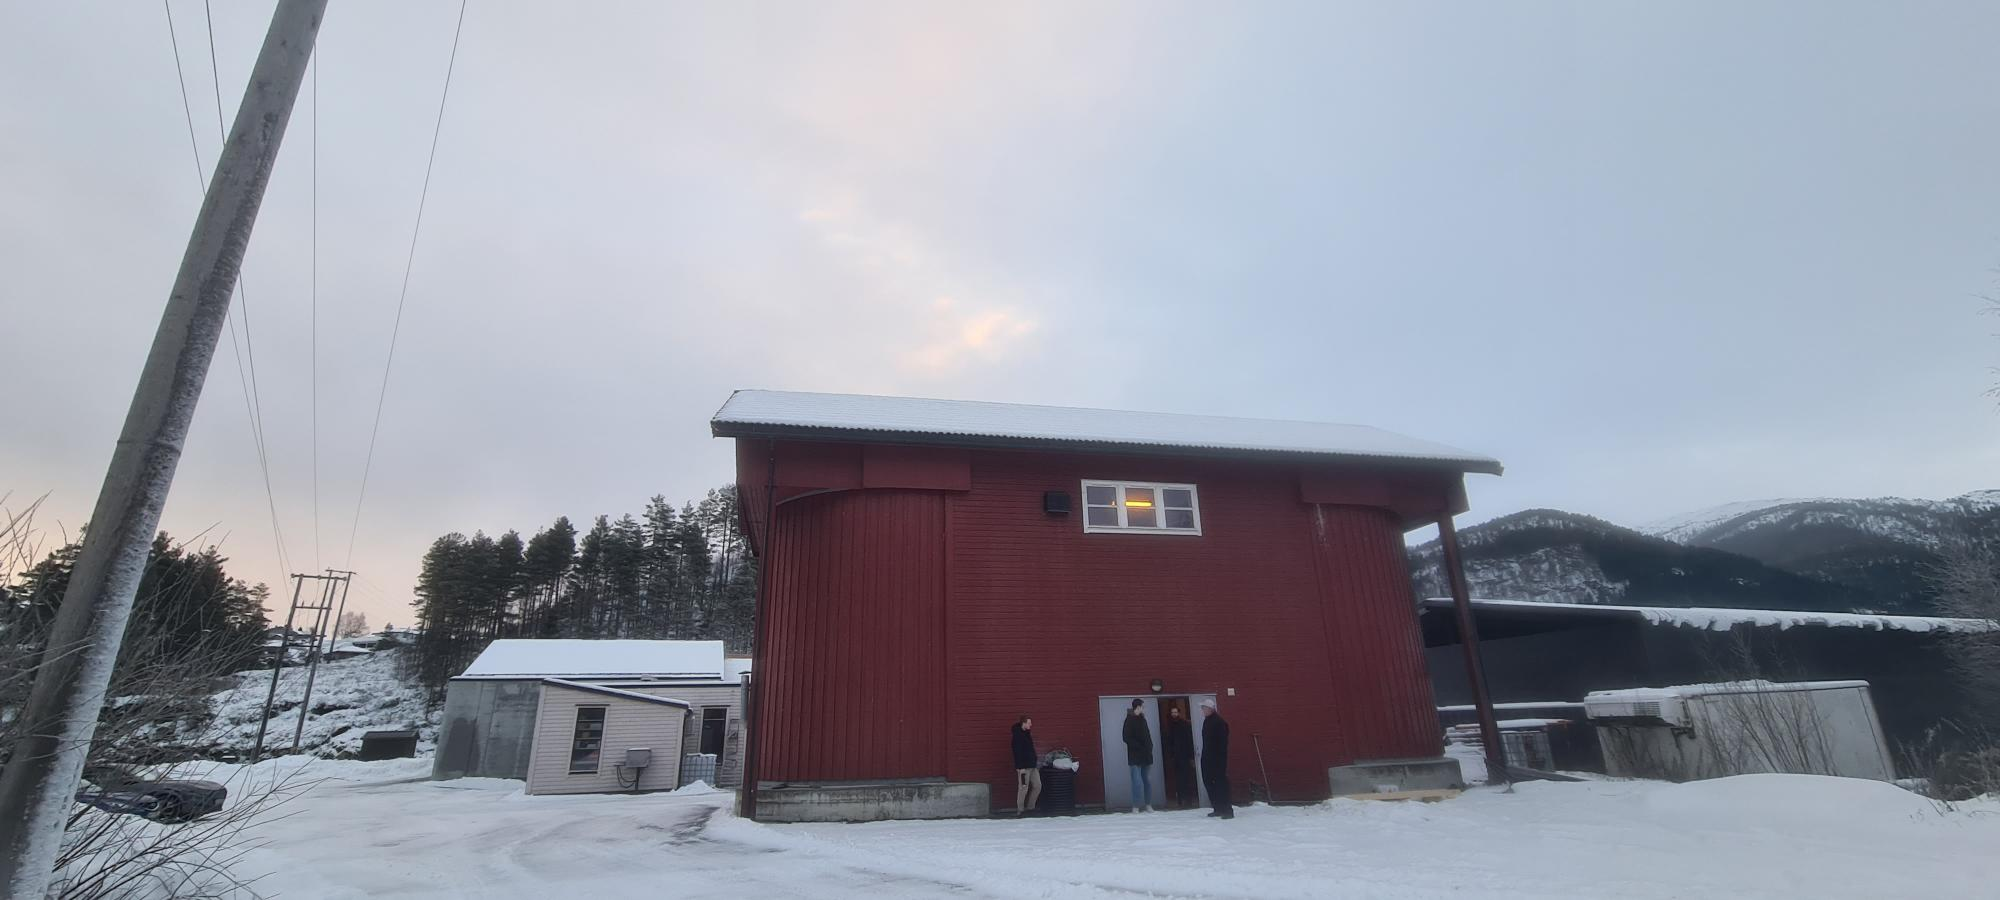
\includegraphics[width=1\textwidth]{Bilder/SandeGjennomgang.jpg}
    \caption{Bilete frå første gjennomgangen av anlegget}\label{fig:Bilete Gjennomgang}
\end{figure}

\begin{center}
    \textit{Foto: Håvar Dankel}
\end{center}

\newpage

\subsection{Anbefalingar sensorikk}

For å forbetre anlegget og styresystemet ytterlegare, vil det vere nyttig å få inn meir instrumentering. 
Meir sensorikk vil forbetre styresystemet ved å samle meir og nøyaktig data om tilstanden og ytelsen til systemet. 
Med auka datamengder vil styresystemet kunne operera meir automatisk og vil kunne tilpassa seg varierande forhold meir effektivt. 
Systemet vil og ha høve til å oppdage avvik og handle tidlegare utan manuelle inngrep, noko som ytterlegare aukar automasjonsevna.

Basert på vår nyerfarte kunnskap om anlegget og styresystemet, presenterer vi ei
anbefaling for oppgradering av instrumentering som vil forbetre reinseanlegget. 
Sjølv om all sensorikk vil være verdifull, har vi vurdert kost-nytte og anbefaler kunn sensorikk som vil gi tilstrekkeleg verdi.


\begin{itemize}
    \item \textbf{Strøymningsmålar} \newline
        Ein Strøymningsmålar i anlegget vil gi nøyaktige mål på mengde vatn som er i anlegget.
        Dette vil forbetre kontrollen på aktivering av høgbelastningsmodus samt kontroll og rapportering av driftsdata.
        Strøymningsmålar er moglege men minimumsanbefalinga er på vatn inn og ut av anlegget.
    \item \textbf{Energimåling} \newline
        Energimåling vil gi moglegheiter for å analysere energiforbruket for å redusere kostnader og effektivisere prosessar.
        Energimåling spesifikt for ulike komponentar kan også brukast til overvåking av utstyr for å oppdage slitasje og feil.
    \item \textbf{Reaktormålingar} \newline
        Målingar av oksygen, pH og temperatur er kritiske for å oppnå god biologisk reinsing i reaktorane.\newline
        Ved å ha kontroll på desse parameterane vil reaktoren kunne finjusterast for å effektivisere den biologiske reinseprosessen.
    \item \textbf{Tilbakemeldingar} \newline
        Anlegget har begrensa tilbakemeldingar frå utstyr, spesielt innan ventilstyring.
        Tilbakemeldingar er essensielt for prosess-styring, feiloppdaging og sikkerheit.
        Utan tilbakemeldingar er reinseanlegget meir sårbar for feil som ikkje blir oppdaga før det er for seint, 
        og slike situasjonar vil kunne resultere i nedetid, overlaup og andre utilsikta hendelser.
    \item \textbf{Forbetra nivåmåling} \newline
        Forbetring av dei eksisterande nivåmålingane i anlegget vil gi meir nøyaktige mål på slammengde og slamnivå i reaktorane.
        Dette vil gjere det mogleg å nøyaktig bestemme skillet mellom slam og reinsa vatn etter ein sedimenteringssekvens,
        noko som gir betre oversikt over tilstanden til den biologiske reinseprosessen.
    \item \textbf{Oppløysning} \newline
        Oppløysninga på analoge målingar er idag kun 0-1000 bit på 4-20mA. \newline
        Oppgradering av måleoppløysning vil gjere kvar eksisterande og nye analoge målingar
        meir nøyaktig, som igjen gir moglegheit for betre styring og regulering.
\end{itemize}
\newpage


